%=========================================================
% FPU Pipeline Structure
%=========================================================
\section{FPU Pipeline Structure}

For the mmRISC-1 core, the RV32F/RV32FC (FPU) instructions have an independent pipeline to the CPU (integer). If there are no register conflict between the CPU and the FPU, each pipeline can go on in parallel. The FPU supports IEEE754 normal, sub-normal, infinite, zero, quiet-nan, signaling-nan and positive/negative for each. The supported rounding modes are RNE (Round to Nearest, tied to even), RTZ (Round to Zero), RDN(Round Down towards minus infinite), RUP (Round Up towards plus infinite), RMM (Round to Nearest, ties to Max Magnitude).\\

As shown in Figure \ref{fig:FPUPipeline}, the FPU pipelines consist of a combination of “i” stage, “a” stage, ‘m’ stage and “f” stage. The “i” stage means “initial” that converts 32bit IEEE754 format data in FRx registers to an internal number format in which there are 1bit sign, 12bit exponent and 66bit fraction. May be, this FPU will easily be able to support 64bit double type in the near future. The “a” stage executes addition and subtraction between the internal formats. The “m” stage executes multiplication between the internal formats. The “f” stage means “finalization” that converts the internal number format to 32bit IEEE754 format and stores the result to an FRx register.\\

FADD.S and FSUB.S instructions consist of “i”, “a” and “f” stages. FMUL.S instruction consists of “i”, “m” and “f” stages. Among FADD.S, FSUB.S and FMUL.S, these instructions can be executed contiguously without stalls if there are no register conflicts each other.\\

FMADD.S, FMSUB.S, FNMADD.S and FNMSUB.S instructions consist of “i”, “m”, “a” and “f” stages. Among FMADD.S, FMSUB.S, FNMADD.S and FNMSUB.S, these instructions can be executed contiguously without stalls if there are no register conflicts. But, between FADD.S etc. and FMADD.S etc, they use common stages, so these contiguous combination of instructions insert appropriate stalls in the pipeline flow to avoid resource conflict. Also, if there are register conflicts between instructions, appropriate stalls are inserted in the pipeline flow.\\

FDIV.S and FSQRT.S use Goldschmidt's Algorithm, so each pipeline consists of “i”, a combination of multiple “a” and “m”, and a final “f” stage. Each convergence loop counts can be configured by the CSR FCONV. For the default configuration, the execution cycle of FDIV.S is 11, and FSQRT.S is 19.\\

Pipelines of instructions to load and store FRn (FLW, FSW) are just same as CPU ones.\\
Pipelines of instructions to convert between integer and float (FCVT.W.S, FCVT.WU.S, FCVTS.W and FCVT.S.WU) consist of “i” stage and “c” stage which is a dedicated stage for conversion.\\
Pipelines of instruction for operations between FRn and FRn (FSGNJ.S, FSGNJN.S, FSGNJX.S, FMIN.S and FMAX.S) and operations between FRn and XRn (FMV.X.W, FMV.W.X, FCLASS.S, FEQ.S, FLT.S and FLE.S) complete in only “i” stage which has almost same meaning as “E” stage of CPU.\\

Detail FPU pipeline logic structure is shown in Figure \ref{fig:FPUPipelineLogicStructure}.\\

\begin{figure}[H]
    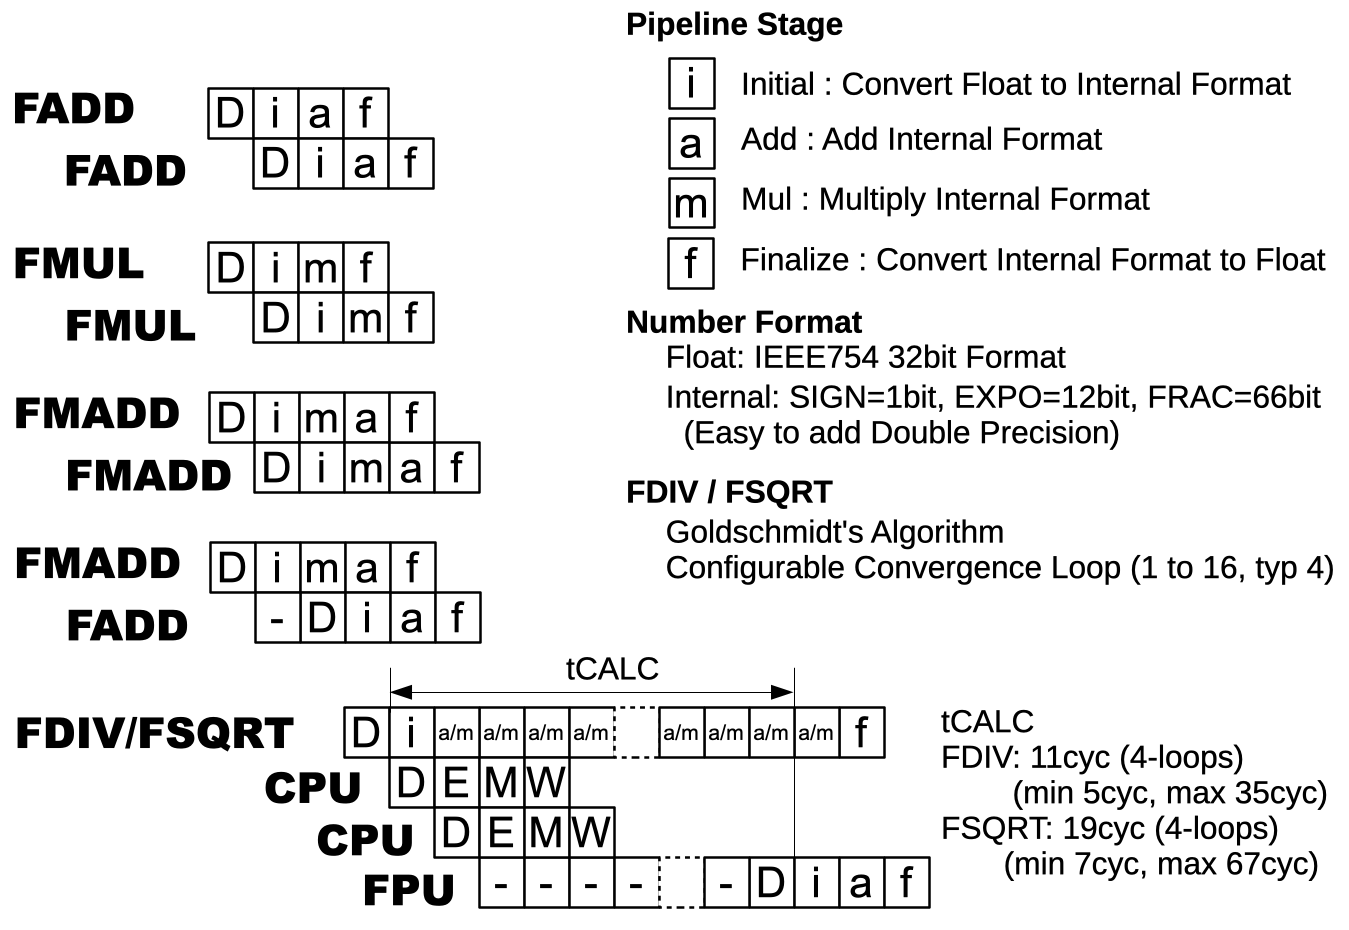
\includegraphics[width=1.00\columnwidth]{./Figure/FPUPipeline.png}
    \caption{FPU Pipeline}
    \label{fig:FPUPipeline}
\end{figure}

\begin{figure}[H]
    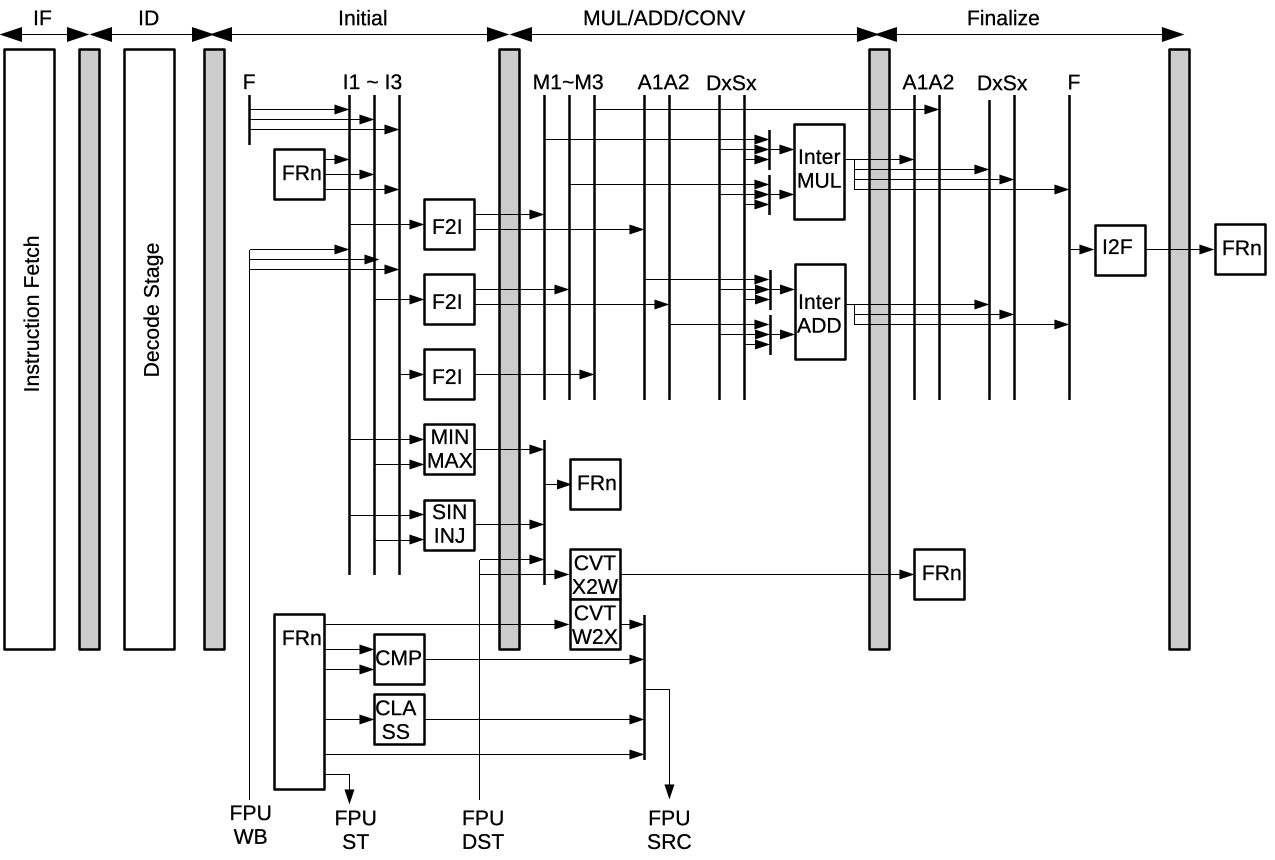
\includegraphics[width=1.00\columnwidth]{./Figure/FPUPipelineLogicStructure.png}
    \caption{FPU Pipeline Logic Structure}
    \label{fig:FPUPipelineLogicStructure}
\end{figure}



